
\de{ĐỀ THI HỌC KỲ I NĂM HỌC 2022-2023}{THPT Nguyễn Hữu Tiến}


%-------------------------
\begin{bt}%[Dự án Đề kiểm tra HKII NH22-23-Nguyễn Văn Sơn]%[THPT NGUYEN HUU TIEN]%[0T3K1-2]
	Tìm tập xác định của các hàm số sau
	\begin{listEX}[2]
		\item $y=\dfrac{x-77}{\sqrt{6-2x}}$.
		\item $y=\dfrac{\sqrt{8-4x}}{\left|1-\sqrt{x-2}\right|}$.
	\end{listEX}
	\dapso{
		a) $\mathscr{D}=\left(-\infty;3\right)$\qquad
		b) $\mathscr{D}=\big\{2\big\}$.
	}
\loigiai
{
	\begin{listEX}
		\item Hàm số xác định khi $6-2x > 0 \Leftrightarrow x < 3$. Tập xác định: $\mathscr{D}=(-\infty; 3)$.
		\item Hàm số xác định khi $\heva{8-4x \geq 0\\ x-2 \geq 0 \\ \sqrt{x-2} \neq 1 }$ $\Leftrightarrow  \heva{x \leq 2\\ x \geq 2 \\ x \neq 3 }$ $\Leftrightarrow x=2$.\\
		Tập xác định: $\mathscr{D}=\big\{2\big\}$
	\end{listEX}
}
\end{bt}

\begin{bt}%[Dự án Đề kiểm tra HKII NH22-23-Nguyễn Văn Sơn]%[THPT NGUYEN HUU TIEN] % [0T3B2-1]
	Cho hàm số $y=-x^2+2x+2$.
	\begin{listEX}
		\item Khảo sát sự biến thiên và vẽ đồ thị hàm số.
		\item Tìm giá trị lớn nhất và giá trị nhỏ nhất của hàm số trên đoạn $[2;\ 3]$.
	\end{listEX}
	\dapso{
		a) 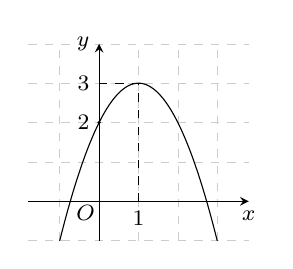
\begin{tikzpicture}[scale=0.5,font=\footnotesize,samples=200,>=stealth]
		\draw[color=gray!40,dashed,very thin] (-1.8,-1) grid (3.8,4);
		\draw[->] (-1.8,0)--(3.8,0) node[below]{$x$};
		\draw[->] (0,-1)--(0,4) node[left]{$y$};
		\node at (0,0) [below left=-2pt]{$O$};
		\clip (-1.4,-1) rectangle (3.4,3.6);
		\draw plot[domain=-1.4:3.4](\x,{-(\x)^2+2*\x+2});
		\fill (0,2) circle(1.3pt) node[left]{$2$};
		\draw[dashed] (1,0)node[below]{$1$}|-(0,3)node[left]{$3$};
		\end{tikzpicture}
		\qquad
		b) $\max\limits_{[2;\ 3]} y=2$ và $\min\limits_{[2;\ 3]} y=-1$.
	}
\end{bt}
\loigiai{
	\begin{listEX}
		\item Khảo sát sự biến thiên và vẽ đồ thị hàm số.\\
		Tập xác định $ \mathscr{D}=\mathbb{R} $.\\
		$y=-x^2+2x+2$ có đỉnh $I(1;3)$.\\
		Trục đối xứng $ x=1 $.\\
		Bảng biến thiên
		\begin{center}
			
\begin{tikzpicture}
				[scale=.8, font=\footnotesize, line join=round, line cap=round, >=stealth]
				\tkzTabInit
				[lgt=2,espcl=3.3] % tùy chọn
				{$x$/1, $y$/2} % cột đầu tiên
				{$-\infty$, $1$, $+\infty$} % hàng 1 cột 2
				\tkzTabVar{-/ $-\infty$, +/ $3$ , -/ $-\infty$} % hàng 3 cột 2
			\end{tikzpicture}
		\end{center}
		Hàm số nghịch biến trên $ (1; +\infty) $ và đồng biến trên $ (-\infty;1) $.\\
		Đồ thị hàm số $y=-x^2+2x+2$\\
		\begin{center} 
			% Đồ thị hàm y=ax^2+bx+c. Nếu hệ số lớn cần điều chỉnh hệ trục, vùng lưới, domain và lệnh \clip
			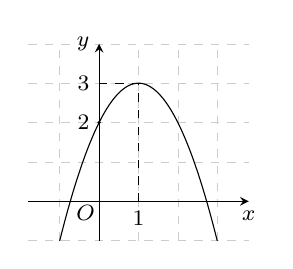
\begin{tikzpicture}[scale=0.5,font=\footnotesize,samples=200,>=stealth]
				\draw[color=gray!40,dashed,very thin] (-1.8,-1) grid (3.8,4);
				\draw[->] (-1.8,0)--(3.8,0) node[below]{$x$};
				\draw[->] (0,-1)--(0,4) node[left]{$y$};
				\node at (0,0) [below left=-2pt]{$O$};
				\clip (-1.4,-1) rectangle (3.4,3.6);
				\draw plot[domain=-1.4:3.4](\x,{-(\x)^2+2*\x+2});
				\fill (0,2) circle(1.3pt) node[left]{$2$};
				\draw[dashed] (1,0)node[below]{$1$}|-(0,3)node[left]{$3$};
			\end{tikzpicture}
		\end{center} 
		\item Tìm giá trị lớn nhất và giá trị nhỏ nhất của hàm số trên đoạn $[2;\ 3]$.\\
		Từ bảng biến thiên ta thấy hàm số nghịch biến trên đoạn $[2;\ 3]$.\\Suy ra $\max\limits_{[2;\ 3]} y=y(2)=2$ và $\min\limits_{[2;\ 3]} y=y(3)=-1$ .\\
	\end{listEX}
	
}
\begin{bt}%[Dự án Đề kiểm tra HKII NH22-23-Nguyễn Văn Sơn]%[THPT NGUYEN HUU TIEN]% [0T3B2-2]
	Xác định parabol $(P)\colon y=ax^2+bx+5$ biết $(P)$ có trục đối xứng $x=2$ và $(P)$ cắt trục hoành tại điểm có hoành độ bằng $-1$.
	\dapso{
		$(P)\colon y=-x^2+4x+5$.
	}
\loigiai{
	Giả thiết suy ra $\heva{&-\dfrac{b}{2a}=2\\& M(-1;0)\in (P)}$ $\Leftrightarrow \heva{4a+b=0&\\a-b=-5&} $$\Leftrightarrow \heva{&a=-1\\&b=4}$.\\
	Ta được parabol $(P)\colon y=-x^2+4x+5$
}
\end{bt}

\begin{bt}%[Dự án Đề kiểm tra HKII NH22-23-Nguyễn Văn Sơn]%[THPT NGUYEN HUU TIEN]% [0T6B3-2]
	Thống kê thời gian học tập tại nhà của $28$ học sinh ngẫu nhiên, ta được kết quả như sau
	
	\hspace{3cm}
	\begin{tabular}{|c|c|c|c|c|c|c|c|c|}
		\hline Thời gian (h) & $0$ & $1$ & $2$ & $3$ & $4$ & $5$ & $6$ & $7$\\
		\hline Số học sinh & $2$ & $4$ & $8$ & $5$ & $5$ & $3$ & $1$ & $0$\\
		\hline
	\end{tabular}
	\begin{listEX}
		\item Tính thời gian trung bình học tập tại nhà của $28$ học sinh này. (Kết quả lấy $2$ chữ số thập phân).
		\item Tìm số trung vị của mẫu số liệu trên.
	\end{listEX}
	\dapso{
		a) $\overline{x}=2{,}7 \mathrm{\,h}$	\qquad
		b) $M_e=2{,}5 \mathrm{\,h}$.
	}
\loigiai{
	\begin{listEX}
	\item $\overline{x}=\dfrac{0 \cdot 2 + 1 \cdot 4 + 2 \cdot 8 + 3 \cdot 5 + 4 \cdot 5 + 5 \cdot 3 + 6 \cdot 1 + 7 \cdot 0}{28}=2 {,}7 \mathrm{\,h}$.
	\item Cỡ mẫu là $n=28$. Khi sắp xếp thời gian học tập tại nhà của học sinh theo thứ tự không giảm thì số liệu thứ $14$ và $15$ lần lượt là $2$ và $3$. Vậy $M_e = \dfrac{1}{2}(2+3)=2 {,}5\mathrm{\,h}$.
	\end{listEX}
}
\end{bt}

\begin{bt}%[Dự án Đề kiểm tra HKII NH22-23-Nguyễn Văn Sơn]%[THPT NGUYEN HUU TIEN] % [0T5B2-5]
	Cho hình vuông $ABCD$ có tâm $O$ và cạnh $AB=a$. Gọi $M$ là trung điểm của cạnh $BC$ và $K$ là một điểm tùy ý.
	\begin{listEX}
		\item Chứng minh rằng $\vec{KA}+\vec{KB}+\vec{KC}+\vec{KD}=4\vec{KO}$.
		\item Tính $\left|\vec{AB}+\vec{AC}\right|$.
	\end{listEX}
	\dapso{
		b) $\left|\vec{AB}+\vec{AC}\right|=4a\sqrt{5}$.
	}
\loigiai{
	\begin{listEX}
		\item Chứng minh rằng $\vec{KA}+\vec{KB}+\vec{KC}+\vec{KD}=4\vec{KO}$.
		\immini{
			\begin{center}
				\begin{tikzpicture}
					\path 
					(0,4) coordinate (A)
					(4,0) coordinate (C)
					(0,0) coordinate (D)
					($(A)+(C)-(D)$) coordinate (B)
					($(A)!.5!(C)$) coordinate (O)
					($(B)!0.5!(C)$) coordinate (M);
					\draw (A)--(B)--(C)--(D)--(A)--(C)--(B)--(D);
					\draw (A)--(M);
					\foreach \x/\y in {A/145,B/45,C/-135,D/-45,O/0,M/0}{\fill (\x) circle(2pt)node[shift={(\y:.35)}]{$\x$};}
				\end{tikzpicture}
			\end{center}
		 }
		
		{
				Ta có $\vec{KA}+\vec{KB}+\vec{KC}+\vec{KD}\\
				=\vec{KO}+\vec{OA}+\vec{KO}+\vec{OB}+\vec{KO}+\vec{OC}+\vec{KO}+\vec{OD}\\
				=4\vec{KO} + \left(\vec{OA}+\vec{OC}\right) +\left(\vec{OC}+\vec{OD}\right)\\
				=4\vec{KO} +\vec{0}+\vec{0}$ (Do $O$ là trung điểm $AC$, $BD$)\\
				$=4\vec{KO}$ (đpcm).
		}
		\item Tính $\left|\vec{AB}+\vec{AC}\right|$.\\
		Ta có $\left|\vec{AB}+\vec{AC}\right|=2\left|\vec{AM}\right|=2AM=2\sqrt{AB^2+BM^2}=2\sqrt{a^2+\left(\dfrac{a}{2}\right)^2}=\sqrt{5}a$.
	\end{listEX}
}
\end{bt}

\begin{bt}%[0T5K4-1]%[Dự án đề kiểm tra HKI NH22-23- Hieu Phan]%[THPT NGUYỄN HỮU TIẾN]
    Cho tam giác $ABC$ có cạnh $AB=4a$, $AC=5a$ và $\cos A=\dfrac{3}{5}$.
    \begin{listEX}
        \item Tính tích vô hướng $\vec{AB} \cdot \vec{AC}$.
        \item Gọi $H$ là trực tâm của $\triangle ABC$ và $M$ là trung điểm của cạnh $BC$. Tính $\vec{MH}\cdot\vec{MA}$.
    \end{listEX}
    \dapso{
        a) $\vec{AB} \cdot \vec{AC}=12a^2$;\qquad
        b) $\vec{MH}\cdot\vec{MA}=\dfrac{17a^2}{4}$.
    }
\loigiai{
 \immini
 {
      \begin{listEX}[1]
      \item Ta có $ \vec{AB} \cdot \vec{AC}=AB\cdot AC\cdot \cos A=4a\cdot 5a\cdot \dfrac{3}{5}=12a^2 $.
      \item Ta có 
      \begin{eqnarray*}
          BC^2&=&AB^2+AC^2-2\cdot AB\cdot AC\cdot\cos A\\
          &=&16a^2+25a^2-24a^2=17a^2.
      \end{eqnarray*} 
  \end{listEX}
 }
 {
     \begin{tikzpicture}[>=stealth,line join=round,line cap=round,line width=0.6pt,font=\footnotesize,scale=1]
         \coordinate[label=below left:$B$](B) at (0,0);
         \coordinate[label=below right:$C$](C) at (4,0);
         \coordinate[label=above left:$A$](A) at (1,3);
         \coordinate (A1) at ($(B)!(A)!(C)$);
         \coordinate (B1) at ($(A)!(B)!(C)$);
         \coordinate (C1) at ($(A)!(C)!(B)$);
          \coordinate (M) at ($(B)!.5!(C)$);
         \draw (A)--(B)--(C)--cycle;
         \draw[blue] (A)--(A1) (B)--(B1) (C)--(C1);
         \path[name path=aa] (A)--(A1);
         \path[name path=bb] (B)--(B1);
         \path[name intersections={of= aa and bb,by=H}];
         \fill (A) circle (1.5pt) (B) circle (1.5pt) (C) circle (1.5pt) (H)node[shift={(-50:10pt)}]{$H$} circle (1.5pt) (M)node[shift={(-50:10pt)}]{$M$} circle (1.5pt);
         \draw ($(A1)!5pt!(C)$)--($(A1)!2!($($(A1)!5pt!(C)$)!.5!($(A1)!5pt!(A)$)$)$)--($(A1)!5pt!(A)$);
         \draw ($(C1)!5pt!(B)$)--($(C1)!2!($($(C1)!5pt!(B)$)!.5!($(C1)!5pt!(C)$)$)$)--($(C1)!5pt!(C)$);
         \draw ($(B1)!5pt!(A)$)--($(B1)!2!($($(B1)!5pt!(A)$)!.5!($(B1)!5pt!(B)$)$)$)--($(B1)!5pt!(B)$);
     \end{tikzpicture}
 }
 \begin{eqnarray*}
    \vec{MH}\cdot\vec{MA}&=&\dfrac{1}{2} \left(\vec{HB}+\vec{HC}\right)\cdot \dfrac{1}{2} \left(\vec{AB}+\vec{AC}\right)\\
    &=&\dfrac{1}{4}\left(\vec{HB}\cdot \vec{AB}+\vec{HB}\cdot \vec{AC}+\vec{HC}\cdot \vec{AB}+\vec{HC}\cdot \vec{AC}\right)\\
    &=& \dfrac{1}{4}\left(\vec{HB}\cdot \vec{AB}+\vec{0}+\vec{0}+\vec{HC}\cdot \vec{AC}\right)\\
    &=&\dfrac{1}{4}\left[\vec{HB}\cdot\left(\vec{AC}+\vec{CB}\right)+\vec{HC}\cdot\left(\vec{AB}+\vec{BC}\right)\right]\\
    &=&\dfrac{1}{4}\left(\vec{HB}\cdot \vec{CB}+\vec{HC}\cdot \vec{BC}\right)=\dfrac{1}{4}\vec{BC}\left(\vec{HC}-\vec{HB}\right)=\dfrac{1}{4}\vec{BC}^2=\dfrac{1}{4}\cdot BC^2=\dfrac{17a^2}{4}.
\end{eqnarray*}
}
\end{bt}

\begin{bt}%[0T4K2-1]%[Dự án đề kiểm tra HKI NH22-23- Hieu Phan]%[THPT NGUYỄN HỮU TIẾN]
    Cho tam giác $ABC$ có $b=8 \mathrm{\,cm}$, $c=5 \mathrm{\,cm}$ và $\widehat{A}=60^{\circ}$.
    \begin{listEX}
        \item Tính độ dài đường cao $h_a$ của tam giác $ABC$.
        \item Tính bán kính $R$ của đường tròn ngoại tiếp tam giác $ABC$.
    \end{listEX}
   \dapso{
    a) $h_a=\dfrac{20\sqrt{3}}{7} \mathrm{\,cm}$;\qquad
    b) $R=\dfrac{7\sqrt{3}}{3} \mathrm{\,cm}$.
}
\loigiai{
\begin{listEX}
    \item Ta có $ S_{\triangle ABC}= \dfrac{1}{2}\cdot b\cdot c\cdot \sin A=\dfrac{1}{2}\cdot 8\cdot 5\cdot \dfrac{\sqrt{3}}{2}=10\sqrt{3}$ $\mathrm{cm^2}$.\\
    Và $ a=\sqrt{8^2+5^2-2\cdot 8\cdot 5\cdot \dfrac{1}{2}} =7$.\\
    Mặt khác  $S_{\triangle ABC}= \dfrac{1}{2}\cdot a
    \cdot h_a  \Rightarrow h_a=\dfrac{2S}{a}=\dfrac{20\sqrt{3}}{7}$ cm.
    \item Ta có $ S=\dfrac{abc}{4R}\Rightarrow R=\dfrac{abc}{4S}=\dfrac{7\cdot 8\cdot 5}{4\cdot 10\sqrt{3}}=\dfrac{7\sqrt{3}}{3}$ cm.
\end{listEX}
}
 
\end{bt}

\begin{bt}%[0T4G3-1]%[Dự án đề kiểm tra HKI NH22-23- Hieu Phan]%[THPT NGUYỄN HỮU TIẾN]
    \immini{
        Người ta định lát gạch tổ ong trên mảnh đất hình tứ giác $ABCD$ như mô hình bên cạnh. Biết rằng $AB=6 \mathrm{\,m}$, $BC=CD=4 \mathrm{\,m}$, $\widehat{ABC}=100^{\circ}$, $\widehat{BCD}=120^{\circ}$ và giá lát gạch là $400$ nghìn đồng trên một mét vuông bao gồm cả công thợ. Hỏi người ta cần bao nhiêu tiền để lát gạch cả mảnh đất đó?}
    {\vspace{-0.5cm}
        \begin{tikzpicture}[scale=1,font=\footnotesize,line join=round,line cap=round]
            %---------------------------
            \foreach \x/\y/\t in {0/0/B,2/0/C}
            \coordinate (\t) at (\x,\y);
            \coordinate (A) at (100:3);
            \coordinate (D) at ($(C)+(60:2)$);
            \draw[thick] (A)--(B)--(C)--(D)--(A);
            \foreach \t/\g in {A/150,B/-150,C/-50,D/10}
            \draw[fill=black] (\t)circle(0.8pt) +(\g:7pt)node{$\t$};
            \begin{scope}[xshift=-0.3cm]
                \pgfmathsetmacro{\r}{0.35};
                \pgfmathsetmacro{\c}{\r*(sqrt 3)/3};
                \node at ($(A)!1/2!(B)$)[left]{$6$};
                \node at ($(C)!1/2!(B)$)[below]{$4$};
                \node at ($(D)!1/2!(C)$)[right]{$4$};
                \clip (A)--(B)--(C)--(D)--(A);
                \foreach \n in {0,1,...,6}
                \foreach \m in {0,1,...,11}{
                    \draw[thin] (\m*\r,\n*3*\c)--++(-150:\c)--++(150:\c)--++(90:\c)--++(30:\c);
                    \draw[thin] (\m*\r,\n*3*\c)--++(-150:\c)--++(-90:\c)--++(-30:\c);}
            \end{scope}
        \end{tikzpicture}
    }
  \dapso{
    $T=\dfrac{1}{2}\left(24\sqrt{3}\sin 70^{\circ}+16\sin 120^{\circ}\right)\cdot 400\,000 \approx 10\,583\,739 $ đồng.
}
\loigiai{
\immini
{ 
    Ta có  \begin{eqnarray*}
        BD&=&\sqrt{BC^2+CD^2-2\cdot BC\cdot CD \cos \widehat{BCD}}\\
        & =&\sqrt{4^2+4^2+2\cdot 4\cdot 4 \cdot \dfrac{1}{2} } =4\sqrt{3}.
    \end{eqnarray*}
    $\triangle BCD$ cân suy ra $\widehat{CBD}=30^\circ\Rightarrow \widehat{ABD}=100^\circ -30^\circ=70^\circ $.
}
{
      \begin{tikzpicture}[scale=1,font=\footnotesize,line join=round,line cap=round]
        %---------------------------
        \foreach \x/\y/\t in {0/0/B,2/0/C}
        \coordinate (\t) at (\x,\y);
        \coordinate (A) at (100:3);
        \coordinate (D) at ($(C)+(60:2)$);
        \draw[thick] (A)--(B)--(C)--(D)--(A);
        \foreach \t/\g in {A/150,B/-150,C/-50,D/10}
        \draw[fill=black] (\t)circle(0.8pt) +(\g:7pt)node{$\t$};
        \begin{scope}[xshift=-0.3cm]
            \pgfmathsetmacro{\r}{0.35};
            \pgfmathsetmacro{\c}{\r*(sqrt 3)/3};
            \node at ($(A)!1/2!(B)$)[left]{$6$};
            \node at ($(C)!1/2!(B)$)[below]{$4$};
            \node at ($(D)!1/2!(C)$)[right]{$4$};
            \draw (A)--(B)--(C)--(D)--(A) (B)--(D);
        \end{scope}
    \end{tikzpicture}
}
  \noindent Ta có $ S_{ABCD}=S_{ABD}+S_{BCD}=\dfrac{1}{2}\left(24\sqrt{3}\sin 70^{\circ}+16\sin 120^{\circ}\right) $.\\
   Vậy số tiền cần để lát gạch cả mảnh đất là
   $$ T=\dfrac{1}{2}\left(24\sqrt{3}\sin 70^{\circ}+16\sin 120^{\circ}\right)\cdot 400\,000 \approx 10\,583\,739 \text{ đồng}. $$
}
  
\end{bt}